% chktex-file -2
\section{Lexical and Syntactical Analysis}

As previously mentioned, the first step during compilation or program execution is the \emph{lexical} and \emph{syntactical analysis}.
Program source text is, without previous processing, just \emph{text} i.e., a sequence of characters.
Before the computer can even begin to analyze the semantics and meaning of a program it has to first \emph{parse} the program source text into an appropriate data structure.
This is done in two steps that are closely related and often combined, the \emph{lexical analysis} performed by a \emph{lexer} and the \emph{syntactical analysis} performed by a \emph{parser}.

\subsection{Formal Syntactical Definition by a Grammar}

Just like every natural language, most programming languages also conform to a grammar.
However, grammars for programming languages most often are of type 2 or 3 in the Chomsky hierarchy, that is \emph{context-free} and \emph{regular} languages, whereas natural languages often are type 1 or 0.
\TODO{citation}
Additionally, it is not uncommon for parser writers to formally define the grammar using some notation.
Popular options include \emph{BNF}\footnote{Backus-Naur Form, named after the two main inventors~\cite{Backus1960}} and \emph{EBNF}\footnote{Extended Backus-Naur Form, an extended version of \emph{BNF} with added support for repetitions and options without relying on recursion, first proposed by Niklaus Wirth in 1977~\cite{Wirth1977} followed by many slight alterations. The version used in this paper is defined by the ISO/IEC 14977 standard.}, the latter of which we use here.
This paper does not further explain these notations, however Listing~\ref{lst:ebnf_reference_grammar} shows a short example grammar notated using EBNF.
For reference, Appendix~\ref{apx:grammar} contains the full grammar of rush.
\TODO{example for type 1 language?}
\TODO{explain start symbol}
\TODO{formal definition of grammars?}
\TODO{explain 1+ repetitions due to `-'}

\Lirsting[float=h, caption={Grammar for Basic Arithmetic in EBNF Notation}, label={lst:ebnf_reference_grammar}]{listings/ebnf_reference.ebnf}

\subsection{Grouping of Characters Into Tokens}

Before the syntax of a program is validated it is common to have a lexer group certain sequences of characters into \emph{tokens}.
The set of tokens a language has is the union of the set of all terminal symbols used in context-free grammar rules and the set of regular grammar rules.
For the language defined in Listing~\ref{lst:ebnf_reference_grammar} these are the five operators `\Verb{+}', `\Verb{-}', `\Verb{*}', `\Verb{/}', `\Verb{**}', and the `integer' non-terminal.

The specifics of implementing a lexer are not explored in this paper, however a basic overview is still provided.
The base principal of a lexer is to iterate over the characters of the input to produce tokens.
Depending on the target language it might however be required to scan the input using an $n$-sized window i.e., observing $n$ characters at a time.
In the case of rush this $n$ is 2, resulting in the \Verb{Lexer} struct not only storing the current character but also the next character as seen in Listing~\ref{lst:lexer}.
For clarity, Table~\ref{tbl:lexer} shows the values of \Verb{curr_char} and \Verb{next_char} during processing of the input `\Verb{1+2**3}'.
Here every row in the table represents one point in time displaying the lexer's current state.
% Listing~\ref{lst:lexer} shows the \Verb{Lexer} struct as it is defined in rush.
% The \Verb{reader} is an iterator over the input characters, the \Verb{location} saves the current index, column, and line in the source text, and the \Verb{curr_char} and \Verb{next_char} fields holds\ldots

% TODO: why does using \Verb inside caption break compilation for @MikMuellerDev
\Lirsting[ranges={10-16}, float=t, caption={The rush \texttt{Lexer} Struct Definition}, label={lst:lexer}]{deps/rush/crates/rush-parser/src/lexer.rs}

\begin{table}[h]
	\newcommand{\lexerframe}[8][]{\tikz[baseline={(frame.base)}]{
			\node(frame)[stack=6, rectangle split part fill={#2}, #1]{
				\texttt{#3}
				\nodepart{two}\texttt{#4}
				\nodepart{three}\texttt{#5}
				\nodepart{four}\texttt{#6}
				\nodepart{five}\texttt{#7}
				\nodepart{six}\texttt{#8}
			};
			% fix margin around tikzpicture
			\node[fit={(current bounding box)}, inner ysep=.5mm, inner xsep=0]{};
		}}
	\centering
	\caption{Advancing Window of a Lexer}\label{tbl:lexer}
	\begin{tabularx}{0.95\textwidth}{rCLLl}
		Calls & State                                                                                                                                                     & \colorbox{black!20}{\Verb{curr_char}} & \colorbox{black!10}{\Verb{next_char}} & Output Token  \\
		\\[-1.1em]\hline\\[-1.1em]
		0     & \lexerframe{none}{1}{+}{2}{*}{*}{3}                                                                                                                       & \Verb{None}                           & \Verb{None}                           &               \\
		0     & \lexerframe{black!10,none}{\bfseries1}{+}{2}{*}{*}{3}                                                                                                     & \Verb{None}                           & \Verb{Some('1')}                      &               \\
		0     & \lexerframe{black!20,black!10,none}{\bfseries1}{\bfseries+}{2}{*}{*}{3}                                                                                   & \Verb{Some('1')}                      & \Verb{Some('+')}                      &               \\
		1     & \lexerframe{none,black!20,black!10,none}{\color{black!50}1}{\bfseries+}{\bfseries2}{*}{*}{3}                                                              & \Verb{Some('+')}                      & \Verb{Some('2')}                      & \Verb{Int(1)} \\
		2     & \lexerframe{none,none,black!20,black!10,none}{\color{black!50}1}{\color{black!50}+}{\bfseries2}{\bfseries*}{*}{3}                                         & \Verb{Some('2')}                      & \Verb{Some('*')}                      & \Verb{Plus}   \\
		3     & \lexerframe{none,none,none,black!20,black!10,none}{\color{black!50}1}{\color{black!50}+}{\color{black!50}2}{\bfseries*}{\bfseries*}{3}                    & \Verb{Some('*')}                      & \Verb{Some('*')}                      & \Verb{Int(2)} \\
		4     & \lexerframe{none,none,none,none,black!20,black!10}{\color{black!50}1}{\color{black!50}+}{\color{black!50}2}{\color{black!50}*}{\bfseries*}{\bfseries3}    & \Verb{Some('*')}                      & \Verb{Some('3')}                      &               \\
		4     & \lexerframe{none,none,none,none,none,black!20}{\color{black!50}1}{\color{black!50}+}{\color{black!50}2}{\color{black!50}*}{\color{black!50}*}{\bfseries3} & \Verb{Some('3')}                      & \Verb{None}                           & \Verb{Pow}    \\
		5     & \lexerframe{none}{\color{black!50}1}{\color{black!50}+}{\color{black!50}2}{\color{black!50}*}{\color{black!50}*}{\color{black!50}3}                       & \Verb{None}                           & \Verb{None}                           & \Verb{Int(3)} \\
	\end{tabularx}
\end{table}

As explained in Section~\ref{sec:stages_of_compilation}, many modern language implementations have the lexer produce tokens on demand.
Thus, a lexer requires one public method called something like \Verb{next_token} reading and returning, as the name suggests, the next token.
In Table~\ref{tbl:lexer} the column on the left displays how many times the \Verb{next_token} method has been called by the parser.
In the first three rows this count is still 0, as this happens during initialization of the lexer in order to fill the \Verb{curr_char} and \Verb{next_char} fields with sensible values before the first token in requested.
The \Verb{Pow} token, composed of two `\Verb{*}' symbols, requires the lexer to advance two times before it can be returned, which is represented by the two rows in which the call count is 4.
A simplified \Verb{Token} struct definition for the example language from Listing~\ref{lst:ebnf_reference_grammar} is shown in Listing~\ref{lst:token_simple}.

\Lirsting[float=h, caption={Simplified \texttt{Token} Struct Definition}, label={lst:token_simple}]{listings/token_simple.rs}

In addition to the current and next character, a lexer also has to keep track of the current position in the source text for it to provide helpful diagnostics with locations to the user.
This is done in the \Verb{location} field which is incremented every time the lexer advances to the next character.
While producing a token the lexer can then read this field once at the start and once after having read the token and save the two values in the token's span.

A special case worth mentioning are comments.
As explained later in Section~\ref{sec:constructing_a_tree}, depending on the parser, comments may be simply ignored and skipped during lexical analysis, or get their own token kind and be treated similar to string literals.

\TODO{maybe mention having spans inclusive or exclusive}

\subsection{Constructing a Tree}\label{sec:constructing_a_tree}

The parser uses the generated tokens in order to construct a tree representing the program's syntactic structure.
Depending on how the parser should be used, this can either be a \emph{Concrete Syntax Tree} (CST) or an \emph{Abstract Syntax Tree} (AST).
The former still contains information about all input tokens with their respective locations, whilst the latter only stores the abstract program structure with just the relevant information for basic analysis and execution.
Therefore, a CST is usually used for development tools like formatters and intricate linters and analyzers where it is important to preserve stylistic choices made by the programmer or to know the exact location of every token.
However, an AST is enough for interpretation and compilation as it preserves the semantic meaning of the program.
Figure~\ref{fig:parser_simple_ast} shows an AST for the program `\Verb{1+2**3}' in the language notated in Listing~\ref{lst:ebnf_reference_grammar} on page~\pageref{lst:ebnf_reference_grammar}.
In the case of rush an AST with limited location information is used, because rush's semantic analyzer is still basic enough to work with that, and, as discussed, execution and compilation requires no CST.

\begin{wrapfigure}{R}{0.5\textwidth}
	\centering
	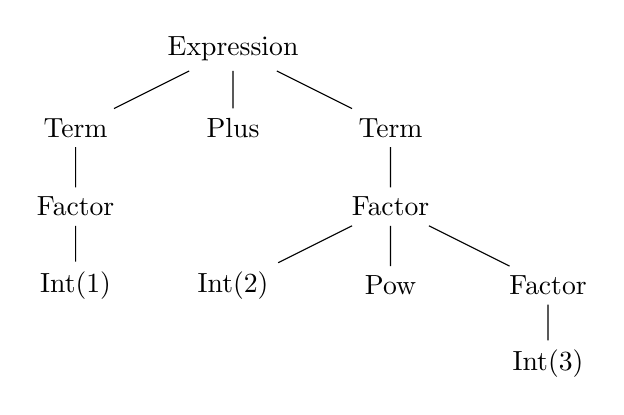
\begin{tikzpicture}[level distance=1cm, sibling distance=2cm]
		\node {Expression}
		child {node {Term}
				child {node {Factor}
						child {node {\Verb{Int(1)}}}}}
		child {node {\Verb{Plus}}}
		child {node {Term}
				child {node {Factor}
						child {node {\Verb{Int(2)}}}
						child {node {\Verb{Pow}}}
						child {node {Factor}
								child {node {\Verb{Int(3)}}}}}};
	\end{tikzpicture}
	\caption{Abstract Syntax Tree for `\texttt{1+2**3}'}\label{fig:parser_simple_ast}
\end{wrapfigure}

Not every parser is the same and there are a few different strategies for implementing one.
These strategies are categorized into \emph{top-down parsers} and \emph{bottom-up parsers}.
The main difference between them being the kind of tree traversal they perform.
Top-down parsers construct the syntax tree in a pre-order manner, meaning a parent node is always processed before its children nodes.
Hence, the syntax tree is constructed from top to bottom, starting with the root node.
Bottom-up parsers instead perform post-order traversal.
That way, all child nodes are processed before their parent node.
This results in the tree being constructed from the leafs at the bottom upwards to the root.

Top-down and bottom-up parsers are further categorized into many more subcategories.
The two we will focus on here are \emph{LL$(k)$} parsers and \emph{LR$(k)$} parsers.
\TODO{`we will' ok?}
\TODO{citation for naming convention}
These are named after the direction of reading the tokens, `L' being from left to right, and the derivation they use.
`L' is the leftmost derivation and `R' the rightmost derivation.
\TODO{what are derivations? + citation}
The parenthesized $k$ represents a natural number with $k\in\mathbb{N}_0$ describing the number of tokens for \emph{lookahead}.
Often $k$ is either $1$ or $0$ for a two or one wide window respectively.
This window moves just like previously explained for the lexer, and observes $k$ \textbf{tokens}, not characters, simultaneously.
Since in most cases $k$ is $1$, it is common to omit specifying it and to just speak of `LL' and `LR' parsers.
\TODO{mention backtracking}

An example for LR parsing is the \emph{shift-reduce} parsing approach.
\ldots\TODO{explain shift-reduce parsing?}\ldots

LL parsers are usually much simpler to implement, but come with a limitation.
By design, they must recognize a node by its first $n=k+1$ tokens, where $n$ is the window size.
However, due to that restriction, not every context-free language can be parsed by \textcolor{red}{a/an} LL parser.
An example for that is given in Listing~\ref{lst:ebnf_reference_pratt}.

\Lirsting[float=h, caption={Example Language a Traditional LL$(1)$ Parser Cannot Parse}, label={lst:ebnf_reference_pratt}]{listings/ebnf_reference_pratt.ebnf}

Most LL parsers are \emph{recursive-descent} parsers, including the rush parser.
Implementation of such a recursive-descent parser is rather uncomplicated.
Assuming the grammar respects the mentioned limitation, every context-free grammar rule is mapped to one method on a \Verb{Parser} struct.
In the example grammar from Listing~\ref{lst:ebnf_reference_grammar} on page~\pageref{lst:ebnf_reference_grammar} again, these are all the capitalized rules highlighted in yellow.
Additionally, a matching node type is defined for each context-free rule, holding the relevant information for execution.
In Rust the mapping from EBNF grammar notation to type definitions is very simple as displayed in Table~\ref{tbl:ebnf_to_rust}.
\TODO{struct signature example}

\begin{table}[h]
	\caption{Mapping From EBNF Grammar to Rust Type Definitions}\label{tbl:ebnf_to_rust}
	\rowcolors{2}{gray!25}{white}
	\begin{tabularx}{0.95\textwidth}{Ll}
		\rowcolor{gray!50} EBNF                         & Rust                                                                         \\
		\hline
		\LirstInline{ebnf}{A = B , C ;}                 & \LirstInline{rs}{struct A { b: B, c: C }}                                    \\
		\LirstInline{ebnf}{A = B , [ C ] ;}             & \LirstInline{rs}{struct A { b: B, c: Option<C> }}                            \\
		\LirstInline{ebnf}{A = B , { C } ;}             & \LirstInline{rs}{struct A { b: B, c: Vec<C> }}                               \\
		\LirstInline{ebnf}{A = B , { C }- ;}            & \LirstInline{rs}{struct A { b: B, c: Vec<C> }}                               \\
		\LirstInline{ebnf}{A = B | C ;}                 & \LirstInline{rs}{enum A { B(B), C(C) }}                                      \\
		\LirstInline{ebnf}{A = B , ( '+' | '-' ) , C ;} & \gape{\makecell[l]{\LirstInline{rs}{struct A { b: B, op: Op, c: C }}         \\\LirstInline{rs}{enum Op { Plus, Minus }}}} \\
		\LirstInline{ebnf}{A = B , [ ( X | Y ) , C ] ;} & \gape{\makecell[l]{\LirstInline{rs}{struct A { b: B, c: Option<(XOrY, C)> }} \\\LirstInline{rs}{enum XOrY { X(X), Y(Y) }}}} \\
	\end{tabularx}
\end{table}

\subsubsection{Operator Precedence}

As previously discussed, a traditional LL parser cannot parse the language from Listing~\ref{lst:ebnf_reference_pratt}.
However, when comparing it to Listing~\ref{lst:ebnf_reference_grammar} it might become obvious that the two grammars notate the same language.
The first one simply provides additional information about the order of nesting different kinds of expressions, called \emph{precedence}.
For example, when parsing the expression `\Verb{1+2*3}' the `\Verb{2*3}' part should be nested deeper in the tree for it to be evaluated first.
In Listing~\ref{lst:ebnf_reference_grammar} this is achieved by recognizing multiplicative expressions as \Verb{Term}s and having additive expressions be composed of \Verb{Term}s.
Listing~\ref{lst:ebnf_reference_pratt} does not indicate the order of evaluation itself, so it must be provided externally.

Additionally, a precedence may be either left or right associative.
Consider the input `\Verb{1*2*3}' it should be evaluated from left to right, so first `\Verb{1*2}' and then the result times 3.
Now consider `\Verb{1**2**3}'\footnote{`\Verb{**}' is the power operator here, so the input would be written as $1^{2^3}$ using mathematical notation}.
Here the `\Verb{2**3}' should be evaluated first and afterwards 1 should be raised to the result.
That means while most operators are evaluated from left to right, that is, they are left associative, some operators like the power operator are evaluated from right to left and are therefore right associative.
In Listing~\ref{lst:ebnf_reference_grammar} left associativity is achieved by allowing simple repetition of the operator for an indefinite amount of times.
Right associativity instead uses recursion on the right-hand side of the operator.

\begin{wrapfigure}{R}{0.5\textwidth}
	\centering
	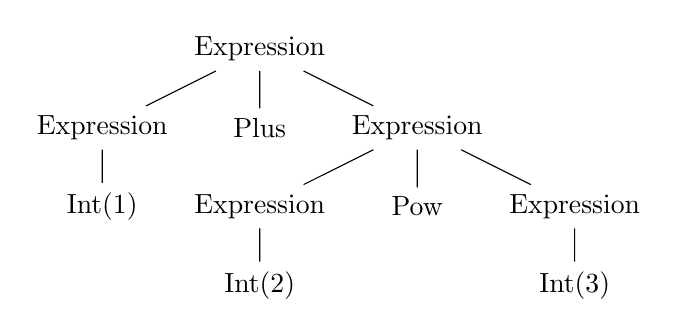
\begin{tikzpicture}[level distance=1cm, sibling distance=2cm]
		\node {Expression}
		child {node {Expression}
				child {node {\Verb{Int(1)}}}}
		child {node {\Verb{Plus}}}
		child {node {Expression}
				child {node {Expression}
						child {node {\Verb{Int(2)}}}}
				child {node {\Verb{Pow}}}
				child {node {Expression}
						child {node {\Verb{Int(3)}}}}};
	\end{tikzpicture}
	\caption{Abstract Syntax Tree for `\texttt{1+2**3}' Using Pratt-Parsing}\label{fig:parser_simple_ast_pratt}
\end{wrapfigure}

For LR parsers the precedence and associativity for each operator is encoded within the parser table.
However, there is also a method called \emph{Pratt-Parsing} that allows slightly modified recursive-descent LL parsers to parse such languages, given a map from tokens to precedences and their associativity.
Often the grammars without included precedence are preferred, because they usually result in a simpler structure of the resulting syntax tree.
This can be seen when comparing Figure~\ref{fig:parser_simple_ast} from earlier to Figure~\ref{fig:parser_simple_ast_pratt} which shows the resulting AST for the same input using the alternative language representation.
Most notably, the rather long sequences of nodes with just a single child, like the path on the left simply resolving to a single \Verb{Int(1)} token, are gone in Figure~\ref{fig:parser_simple_ast_pratt}.

\subsubsection{Pratt-Parsing}

As the rush parser makes use of Pratt-Parsing, most of the following code snippets are taken from there.
First a mapping from a token kind to its precedence must be defined.
The one for rush is found in Listing~\ref{lst:rush_tok_prec}.
It shows the \Verb{prec} method implemented on the \Verb{TokenKind} enum.
The return type is a tuple of two integers, one for left and one for right precedence.
For all but one token kind the left precedence is lower than the right one, resulting in left associativity.
The higher the precedences are, the deeper in the tree the resulting expressions will be, and the earlier they are evaluated.
All unrelated tokens are simply assigned a precedence of 0 for left and right.

\Lirsting[ranges={172-173, 194-201}, float=h, label={lst:rush_tok_prec}, caption={Token Precedences in rush}, gobble=4]{deps/rush/crates/rush-parser/src/token.rs}

The \Verb{expression} method on the \Verb{Parser} struct is then modified to take a parameter for the current precedence as seen in Listing~\ref{lst:pratt_expr}.
It then first matches on the current token kind to decide which expression to parse and stores the result in the \Verb{lhs}\footnote{Short for `left-hand side'} variable.
Afterwards it checks whether the left precedence of the now current token is bigger than the \Verb{prec} argument.
When called from elsewhere, like in the condition of a while-loop or in a grouped expression, the \Verb{prec} argument has its minimum value of 0 as shown in Listing~\ref{lst:pratt_grouped}.
In that case this check will only fail, when the whole expression is over, as every non-operator token is assigned a precedence higher than 0.
If it does not fail, the \Verb{infix_expr} method is called with the matching operator and the \Verb{lhs}.
Afterwards \Verb{lhs} is overwritten with the returned value.
The \Verb{infix_expr} method itself simply stores the right precedence of the operator token, advances to the next token, and calls the \Verb{expression} method again for its right-hand side, but this time with the stored \Verb{right_prec} as the minimum precedence.

\Lirsting[ranges={733-733, 738-738, 749-749}, float=h, label={lst:pratt_grouped}, caption={Pratt-Parser: Call to \Verb{expression} With the Lowest Precedence}, gobble=4]{deps/rush/crates/rush-parser/src/parser.rs}

\Lirsting[ranges={551-555, 568-583, 613-618, 751-759, 770-770}, float=h, label={lst:pratt_expr}, caption={Pratt-Parser Implementation \TODO{split into 2 listings?}}, gobble=4]{deps/rush/crates/rush-parser/src/parser.rs}

\begin{figure}[h]
    \newcommand{\precs}[4][black]{
        \node(#2_lprec)[prec, color=#1, below=of #2, xshift=-4mm]{#3};
        \node(#2_rprec)[prec, color=#1, below=of #2, xshift= 4mm]{#4};
        \draw[arrow, color=#1](#2) -- (#2_lprec);
        \draw[arrow, color=#1](#2) -- (#2_rprec);
    }
	\centering
    \begin{tikzpicture}[node distance=4mm and 1cm, prec/.style={font=\footnotesize}]
		\node(lparen)                 {\Verb{(}};
		\node(1)     [right=of lparen]{\Verb{1}};
		\node(+)     [right=of 1]     {\Verb{+}};
		\node(2)     [right=of +]     {\Verb{2}};
		\node(*)     [right=of 2]     {\Verb{*}};
		\node(3)     [right=of *]     {\Verb{3}};
		\node(rparen)[right=of 3]     {\Verb{)}};
		\node(/)     [right=of rparen]{\Verb{/}};
		\node(4)     [right=of /]     {\Verb{4}};
		\node(**)    [right=of 4]     {\Verb{**}};
		\node(5)     [right=of **]    {\Verb{5}};

        \precs      {lparen}{28}{29}
        \precs[gray]{1}     {0} {0}
        \precs      {+}     {19}{20}
        \precs[gray]{2}     {0} {0}
        \precs      {*}     {21}{22}
        \precs[gray]{3}     {0} {0}
        \precs      {rparen}{0} {0}
        \precs      {/}     {21}{22}
        \precs[gray]{4}     {0} {0}
        \precs      {**}    {26}{25}
        \precs[gray]{5}     {0} {0}
	\end{tikzpicture}
	\caption{Token Precedences for Input `\Verb{(1+2*3)/4**5}`}\label{fig:token_precs}
\end{figure}

\subsubsection{Parser Generators}

For most intents and purposes it is generally not recommended and necessary to implement parsers, and with that lexers, manually.
\TODO{citation}
Instead, there are so-called \emph{parser generators} that generate parsers based on some specification of the desired syntax.
Often parser generators define a domain specific grammar notation for the syntax specification.
\TODO{some also allow traditional grammar notations, and e.g., `nom' is simply a Rust crate}
\ldots

\begin{enumerate}
	\item different strategies (LL, LR) and top-down / bottom-up
	\item lookahead (to avoid backtracking)
	\item pratt-parsing
	\item parser generators
\end{enumerate}
